% Springer Nature manuscript prepared for the International Journal of
% Data Science and Analytics using the supplied sn-jnl class.
\documentclass[pdflatex,sn-mathphys-num,iicol]{sn-jnl}

\usepackage{graphicx}
\graphicspath{{./}}
\usepackage{booktabs}
\usepackage{amsmath,amssymb,amsfonts}
\usepackage{microtype}
% Disable font expansion for compatibility with bitmap fonts in minimal TeX installs.
\microtypesetup{expansion=false}
\usepackage{array}
\usepackage{url}
\setlength{\emergencystretch}{3em}
\raggedbottom

\begin{document}

\title[A Reproducible Event-Fixed Protocol for Evaluating Financial Stress Detectors]{A Reproducible Event-Fixed Protocol for Evaluating Financial Stress Detectors}

\author*[1]{\fnm{Prashant} \sur{Singh}}\email{2023mcb1309@iitrpr.ac.in}


\author[1]{\fnm{Pranav} \sur{Singh}}\email{2023mcb1308@iitrpr.ac.in}


\affil*[1]{\orgdiv{Department of Mathematics}, \orgname{Indian Institute of Technology Ropar}, \orgaddress{\city{Rupnagar}, \postcode{140001}, \state{Punjab}, \country{India}}}

\abstract{Financial stress detectors are conventionally evaluated with day-level classification metrics computed over alarm days. Because this evaluation design is specified before any data are scored, it can determine the ranking of competing detectors independently of their detection ability. We introduce an event-fixed evaluation protocol that fixes a panel of documented U.S. equity stress episodes before any detector output is examined, and that reports day-level classification metrics, event-level detection rates, detection delay, and cost-sensitive loss jointly. Applied on SPY to a volatility percentile trigger and to a confirmation rule requiring an additional instability signal, the ranking of the two detectors reverses across these metric families. The confirmation rule attains a lower false positive rate and higher precision, whereas the trigger attains a higher event-level detection rate and a shorter detection delay. The same reversal holds when a standard implied volatility index replaces the study-specific trigger, indicating a property of the evaluation design rather than of a particular detector. We therefore characterize the trade-off by the cost ratio at which the two detectors incur equal expected loss, and provide a reproducibility package for all reported results.}

\keywords{financial stress detection; event-fixed evaluation; time-series anomaly detection; financial risk monitoring; detection delay; cost-sensitive evaluation}

\maketitle


\section{Introduction}
A detector that raises alarms on few quiet days does not necessarily detect more of the episodes that matter. The ranking of two detectors can therefore depend on whether performance is measured over individual days or over a fixed set of stress episodes, and that choice is made before any data are scored.

This paper proposes an evaluation protocol that fixes the set of stress episodes before any detector output is examined. Each episode is taken from published accounts of stress in the U.S. equity market, given a start and an end date, and mapped to a window of trading days. An episode counts as detected if at least one alarm falls inside its window, and an alarm on a day outside every window counts as a false alarm. The protocol reports performance measured over days and performance measured over episodes together.

We apply the protocol to two detectors on twenty-four years of daily SPY data. The percentile trigger raises an alarm whenever realized volatility exceeds a fixed percentile of its own trailing distribution. The confirmation rule raises an alarm only when that volatility condition is accompanied by an exceedance in a composite instability signal, defined in Section~\ref{sec:method}. The two views rank these detectors in opposite orders. The confirmation rule raises alarms on a smaller fraction of the days outside the episode windows, and more of the alarms it raises fall inside them. The percentile trigger detects more of the episodes, raises its first alarm within an episode sooner, and gives a lower expected loss whenever a false alarm is assigned a small cost relative to a missed episode. Both rankings come from the same two alarm series over the same sample, and differ only in the scoring rule applied to them.

Evaluation is difficult here because stress episodes are rare and their start and end dates are not agreed upon. Volatility often rises before the date conventionally assigned to a crisis and stays high after it, and published studies differ in the dates and window lengths they adopt. Research measuring how prices respond to corporate announcements resolved a comparable problem by requiring that announcement dates be specified before the returns around them are examined \cite{brown1985, mackinlay1997}. Research on benchmarks for anomaly detection in time series shows the opposite risk: the construction of labels and scores can make a method appear better than others without any improvement in detection \cite{lavin2015, wu2022}.

Detection methods for financial time series are numerous, whereas the evaluation layer beneath them has received less scrutiny. It determines which episodes constitute the target, how their windows are built, whether the delay to the first alarm is measured, and how a false alarm is weighted against a missed episode. For rare episodes separated by long quiet periods, one summary metric is not sufficient to rank detectors.

\subsection*{What this paper contributes}
\begin{enumerate}
\item \textbf{An evaluation protocol with the episode set fixed in advance, and evidence that it changes the ranking.} With 13 episodes fixed before any output is inspected, the confirmation rule raises alarms on 0.005 of the days outside the windows against 0.044, and 0.886 of its alarms fall inside a window against 0.640, but it detects 8 of the 13 episodes against 10. Both sets of figures are correct, and each alone supports a different ranking.
\item \textbf{The reversal is not specific to the detector built here.} Replacing the volatility measure with the Cboe Volatility Index, a published index of the volatility that S\&P 500 option prices imply for the following month, and applying the same confirmation condition raises the fraction of alarms falling inside windows from 0.596 to 0.947 and reduces alarm days outside every window from 214 to 9, while episodes detected fall from 10 to 7.
\item \textbf{An explanation of why the ranking reverses.} The composite signal is dominated by a return divided by the volatility of the preceding 50 days, so any rise in volatility that those 50 days absorb enters the divisor and cancels. Across the episodes the confirmation rule detects, the spread of raw volatility rises by a factor of 3.03 and that of the composite by 1.29.
\item \textbf{The cost ratio at which the preferred detector changes.} On SPY the percentile trigger gives the lower expected loss only when one false alarm is assigned a cost below 0.021 of one missed episode, that is, when 48 false alarms are treated as no worse than one missed episode. We report this ratio for five assets and three penalties for late detection.
\item \textbf{Evidence that the reversal does not depend on the parameter values chosen.} The weights combining the components of the composite signal, the number of days allowed between the two conditions, the number of trading days in each episode window, and the sign convention applied to the persistence statistic are each varied in turn, and the reversal persists in every case.
\end{enumerate}

Table~\ref{tab:protocol_comparison} summarizes how the protocol combines elements already established separately in the literature, from fixed episode dates to cost-sensitive interpretation, into one design.

Section~\ref{sec:related} reviews prior work on studies with dates fixed in advance, benchmarks for anomaly detection in time series, early-warning indicators for financial crises, and the backtesting of risk models. Section~\ref{sec:method} defines the protocol and the two detectors. Section~\ref{sec:results} reports the main results, including the comparison against the published volatility index, then sensitivity and auxiliary checks. Sections~\ref{sec:discussion} and~\ref{sec:limits} address interpretation and scope, Section~\ref{sec:repro} reproducibility, and Section~\ref{sec:conclusion} concludes.

\begin{table*}[t]
\centering
\caption{Relationship between established evaluation elements and the event-fixed protocol.}
\label{tab:protocol_comparison}
\scriptsize
\begin{tabular}{p{0.30\linewidth}p{0.62\linewidth}}
\toprule
Established evaluation element & Role in this protocol\\
\midrule
Fixed event panel & Uses a fixed panel of documented U.S. equity-market stress events before detector inspection.\\
Pre-specified inclusion rule & Applies explicit inclusion criteria based on broad market relevance, clear calendar dating, documented sources, and observable equity-market impact.\\
Event-level metrics & Reports whether each documented stress episode is detected, in addition to pointwise precision, recall, F1, and FPR.\\
Delay metrics & Reports FDD and alignment error relative to the mapped event date.\\
Severity organization & Uses realized-drawdown terciles as descriptive categories for organizing event-level interpretation.\\
Multi-asset consistency check & Applies the same protocol without asset-specific detector tuning across equity, credit, and Treasury exchange-traded funds.\\
Cost-sensitive interpretation & Reports pointwise and event-aware operating costs, and the crossover ratio at which the preferred detector changes.\\
Reproducibility package & Provides event definitions, source strings, mapped event tables, configuration, random seed, and reproduction procedure.\\
\bottomrule
\end{tabular}
\end{table*}

\section{Related Work}
\label{sec:related}
Fixing dates before the outcome is examined is an established practice in finance. An event study measures how prices behave around a dated event, and the dates are fixed before any returns are inspected \cite{brown1985, mackinlay1997}. Dates for episodes of financial stress come from published sources a reader can check, such as the NBER recession dates \cite{nber2023}, the Financial Crisis Inquiry Commission report \cite{fcic2011}, and the CFTC--SEC account of the May 2010 Flash Crash \cite{cftcsec2010}. Neither approach was built to score a detector that produces a value every trading day, and neither counts alarms outside an event window, episodes that receive no alarm, or the delay before the first alarm. Benchmarks for anomaly detection do that: they label windows in a stream and score detectors against those labels \cite{lavin2015, ahmad2017}. They also show that the choice of labels can make a method look better without detecting more \cite{wu2022}. These benchmarks are not tied to documented episodes of financial stress.

Two literatures combine both commitments and are the closest precedents for the protocol proposed here. Backtesting of value-at-risk and expected shortfall counts exceptions against a threshold and a horizon fixed in advance: Kupiec tests whether the number of exceptions matches the rate the model claims \cite{kupiec1995}, Christoffersen tests whether exceptions arrive independently rather than in clusters \cite{christoffersen1998}, and the Basel traffic-light framework turns a count over 250 days into a stated supervisory consequence \cite{bcbs1996}. The signals approach to early warning fixes a list of dated currency crises, opens a window before each one, and classifies every threshold crossing as a signal or a false alarm, summarized by the ratio of noise to signal \cite{kaminsky1998}; later work tests that design out of sample \cite{berg1999} and restates it as a loss function weighing missed crises against false alarms \cite{bussiere2006}. In both, the dates and the cost of an error are set before any result is seen, and the unit of account is the exception or the crisis rather than the day. The protocol here carries those commitments to daily detector output, where a monthly binary indicator and a symmetric ratio are not sufficient: it measures the delay to the first alarm in trading days and prices a late confirmation separately from a missed episode, through the cost in Equation~\eqref{eq:eventcost} and the crossover ratio of Section~\ref{sec:cost}.

The detectors compared here are built from standard measurements. Drawdown records how far a price has fallen from its recent peak \cite{magdon2004}, and realized volatility records how much daily returns vary \cite{andersen2003}. Large returns and long runs of high volatility are long-documented features of these series \cite{mandelbrot1963,cont2001,engle1982,bollerslev1986}. Variance and autocorrelation often rise before a regime shift \cite{scheffer2009,dakos2012}, though both are hard to identify in short samples \cite{boettiger2012}; this is what the instability signal is meant to capture. Sequential change-point tests \cite{page1954} and kernel two-sample statistics \cite{gretton2012} are alternatives. Recent applied work uses methods of this kind to predict or monitor stress \cite{gu2024,aldasoro2025,imf2026}. None of it says how the resulting detectors should be compared.

\section{Methodology}
\label{sec:method}
This section defines the evaluation protocol first and the two detectors second. We fix the list of stress episodes, match each episode date to a day on which the asset traded, and group the episodes into descriptive severity categories. We then define what a detector must output, the metrics computed over days and over episodes, the cost model, and the uncertainty summaries. The percentile trigger and the confirmation rule are defined last, because this paper is about the protocol rather than about either detector.

\subsection{Data}
The main analysis uses SPY. Four further assets are used to check that the results are not specific to one series: QQQ, IWM, HYG, and TLT. The comparison against a published volatility index uses the Cboe Volatility Index. All series are daily adjusted closing prices obtained from Yahoo Finance. SPY, QQQ, and the VIX cover 3 January 2000 to 29 December 2023; IWM, TLT, and HYG begin at their inception dates of 26 May 2000, 30 July 2002, and 11 April 2007. Table~\ref{tab:asset_availability} gives the usable sample for each series after preprocessing. The exact files used are archived with the code, so every reported number can be recomputed from the same input. The number of usable days for each asset is given in Appendix~\ref{app:implementation_details}.

Each episode date is matched to the nearest day on which the asset in question traded, separately for each asset, because the five assets do not share every trading day.

\subsection{Signals}
Let $P_t$ be the adjusted closing price on trading day $t$. The detectors read three quantities, all computed from returns:
\begin{align}
r_t &= \log(P_t/P_{t-1}),\\
\sigma_t &= \mathrm{sd}(r_{t-19},\dots,r_t),\\
z_t &= (r_t-\mu_t)/s_t,\\
x_t &= 0.5\,r_t + 0.3\,\sigma_t + 0.2\,z_t.
\end{align}
Here $r_t$ is the return on day $t$. The quantity $\sigma_t$ is the standard deviation of the 20 most recent returns, that is, of returns from day $t-19$ to day $t$; twenty trading days is approximately one month, short enough for $\sigma_t$ to move within an episode. The quantity $z_t$ expresses the day's return in units of recent variation: $\mu_t$ and $s_t$ are the mean and the standard deviation of the 50 most recent returns, and fifty trading days is approximately one quarter, long enough for those two estimates to be stable. Both window lengths are fixed for every result reported.

The composite $x_t$ combines the three into the single number required by the components that compare distributions. The three terms are measured on different scales, so the coefficients $(0.5, 0.3, 0.2)$ do not state how much each term contributes. Over the SPY sample the standard deviations of the three weighted terms are $0.0062$ for $0.5\,r_t$, $0.0020$ for $0.3\,\sigma_t$, and $0.2028$ for $0.2\,z_t$, against $0.2083$ for $x_t$; the correlation between $x_t$ and $z_t$ is $0.9999$. The composite is therefore a rescaled version of $z_t$: each of the other two weighted terms has a standard deviation below 3 per cent of that of $x_t$.

This has a consequence for what the composite can register. Because $z_t$ divides by the standard deviation of the previous 50 returns, a rise in volatility that lasts long enough to enter that window also raises the divisor, and $z_t$ falls back toward its earlier range. The composite responds to a return that is large relative to the previous fifty days, and not to a sustained period of high volatility. The coefficients are held at these values for every result reported and are never chosen using the evaluation data.

\subsection{Which events are included}
The panel of stress events is fixed before any detector output is examined, and no event is added or removed on the basis of what a detector does. An event is included only if it has all four of:
\begin{itemize}
\item a broad effect on U.S. equities, SPY and the S\&P 500 included;
\item a date identifiable to the day and mappable to a trading day;
\item documentation by a public source: a regulator, a central bank, the NBER chronology, an exchange, or a published study;
\item a fall in U.S. equity prices in the daily record.
\end{itemize}
An event is excluded if any of these holds:
\begin{itemize}
\item its date is not identifiable to the day;
\item its effect is confined to one sector or one region;
\item its window would overlap that of an included event.
\end{itemize}
The resulting panel contains 13 events. It is a fixed list for scoring detectors, not a complete chronology of market stress. Its main sources are the NBER recession dates \cite{nber2023}, the report of the Financial Crisis Inquiry Commission \cite{fcic2011}, the CFTC--SEC report on the May 2010 Flash Crash \cite{cftcsec2010}, and Khandani and Lo on the August 2007 losses at quantitative funds \cite{khandani2007}. Table~\ref{tab:events} gives each event with its date, the trading day it is mapped to, and the source used to date it.

\begin{table*}[t]
\centering
\caption{Fixed panel of 13 SPY stress events. Calendar is the documented date and Trading is the day it is mapped to. DD is the drawdown realized inside the event window, and Severity is the tercile of DD within the panel.}
\label{tab:events}
\scriptsize
\setlength{\tabcolsep}{2.5pt}
\begin{tabular}{>{\raggedright\arraybackslash}p{0.028\linewidth}>{\raggedright\arraybackslash}p{0.115\linewidth}>{\raggedright\arraybackslash}p{0.095\linewidth}>{\raggedright\arraybackslash}p{0.095\linewidth}>{\raggedright\arraybackslash}p{0.12\linewidth}>{\raggedright\arraybackslash}p{0.245\linewidth}>{\raggedright\arraybackslash}p{0.048\linewidth}>{\raggedright\arraybackslash}p{0.058\linewidth}}
\toprule
ID & Event & Calendar & Trading & Type & Source label & DD & Severity \\
\midrule
E01 & Dot-com selloff & 2000-04-14 & 2000-04-14 & bear market & Fed History; NBER chronology & 0.114 & high\\
E02 & Sep. 11 reopening & 2001-09-17 & 2001-09-17 & exogenous shock & SEC/NYSE reopening documentation & 0.182 & critical\\
E03 & WorldCom selloff & 2002-07-24 & 2002-07-24 & accounting & SEC WorldCom litigation; Fed History & 0.196 & critical\\
E04 & Quant crisis & 2007-08-09 & 2007-08-09 & liquidity & Khandani--Lo (2007); Fed accounts & 0.090 & medium\\
E05 & Lehman crisis & 2008-09-29 & 2008-09-29 & systemic & FCIC report; NBER chronology & 0.344 & critical\\
E06 & Flash crash & 2010-05-06 & 2010-05-06 & micro\-structure & CFTC--SEC Flash Crash report & 0.123 & high\\
E07 & U.S. downgrade & 2011-08-08 & 2011-08-08 & sovereign credit & S\&P downgrade; Fed commentary & 0.166 & critical\\
E08 & China devaluation & 2015-08-24 & 2015-08-24 & global growth & Fed/BIS market commentary & 0.112 & medium\\
E09 & Volmageddon & 2018-02-05 & 2018-02-05 & volatility & Cboe volatility-product discussion; SEC/CFTC commentary & 0.101 & medium\\
E10 & Q4 2018 selloff & 2018-12-24 & 2018-12-24 & liquidity & Federal Reserve Financial Stability Report & 0.156 & high\\
E11 & COVID crash & 2020-03-16 & 2020-03-16 & pandemic & Fed FSR May 2020; NBER chronology & 0.337 & critical\\
E12 & Inflation selloff & 2022-06-13 & 2022-06-13 & inflation & Federal Reserve Financial Stability Report & 0.122 & high\\
E13 & Bank stress & 2023-03-13 & 2023-03-13 & banking & Fed SVB review; Fed FSR 2023 & 0.069 & medium\\
\bottomrule
\end{tabular}
\end{table*}

\subsection{Event severity}
Each event is assigned a severity, the largest fall in the SPY price inside a window around it. Let $P_t$ be the adjusted closing price on trading day $t$, and let $W_e$ run from 20 trading days before the mapped event day $e$ to 20 trading days after it, about one month on each side. With $M_t=\max_{u\in[e-20,\,t]}P_u$ the highest close up to day $t$, and $D_t=P_t/M_t-1$ the fall of the price below that high,
\begin{equation}
\mathrm{severity}(e)=\Big|\min_{t\in W_e} D_t\Big|.
\end{equation}
As an example, take the dot-com selloff of April 2000 (E01 in Table~\ref{tab:events}). The lowest value of $P_t/M_t$ inside its window is $0.886$, so
\begin{equation}
\mathrm{severity}(\mathrm{E01}) = |0.886 - 1| = 0.114,
\end{equation}
a realized fall of 11.4 per cent, which is the value reported for E01 in Table~\ref{tab:events}.
This is the maximum drawdown \cite{magdon2004} restricted to the event window. The 13 severities are split at their terciles into groups labelled medium, high, and critical. The groups describe the panel, and no reported result depends on them. Severity is computed from SPY for every asset.

\subsection{Event windows}
Alarms are counted over a window running from 60 trading days before the mapped event day to 60 trading days after it, about three months on each side, because stress typically begins before the documented date and continues after it. The window fixes the days over which alarms are counted and is not a statement about when the episode began or ended. An alarm anywhere in the window counts the same, so the delay to the first alarm is reported separately. Windows of 20, 30, and 45 trading days on each side are also evaluated, and the comparison between the two detectors is unchanged at every width.

\subsection{Event-level metrics}
\label{sec:event_metrics}
Day-level metrics count alarm days but do not record whether an event received any alarm. Let $A$ be the set of days on which a detector raises an alarm. For each asset, event, and detector, five quantities are computed over the window $[e-60,\,e+60]$:
\begin{itemize}
\item \textbf{Detection}: 1 if any day of the window lies in $A$, else 0. The detection rate is the mean over the 13 events.
\item \textbf{First-alarm delay}: trading days from $e$ to the earliest alarm in the window, negative if it precedes $e$, undefined if the event is not detected.
\item \textbf{Nearest-alarm delay}: the same count for the alarm closest to $e$ in either direction.
\item \textbf{Coverage}: the fraction of the window's trading days that are alarm days.
\item \textbf{Alarms before and after}: whether any alarm falls in $[e-60,\,e-1]$, and whether any falls in $[e,\,e+60]$.
\end{itemize}

\subsection{Detector definitions}
Every threshold below is set on the first 70 per cent of each asset's daily sample, called the calibration period, and applied unchanged to the whole series. The split fixes each threshold on the earlier part of the sample, so no threshold is chosen using the later data. For any daily score $q_t$, standardization uses the calibration mean and standard deviation,
\begin{equation}
z_q(t)=\frac{q_t-\mu_{q,\mathrm{cal}}}{\sigma_{q,\mathrm{cal}}},
\end{equation}
and smoothing, unless stated otherwise, is the mean of the five most recent values, one trading week,
\begin{equation}
\bar q_t=\frac{1}{5}\sum_{j=0}^{4}q_{t-j},
\end{equation}
taken over the available values at the start of a series.
\begin{itemize}
\item \textbf{Volatility percentile trigger.} Standardize $\sigma_t$, smooth it, and set $v(t)=1$ when the result exceeds its 90th percentile over the calibration period. The input is $\sigma_t$ itself, which is not divided by any trailing scale.
\item \textbf{CUSUM.} From standardized returns $z_r(t)$, accumulate
\begin{align}
C^+_t &= \max(0,\,C^+_{t-1}+z_r(t)),\\
C^-_t &= \min(0,\,C^-_{t-1}+z_r(t)),\\
C_t &= \max(C^+_t,\,-C^-_t),
\end{align}
where $C_t$ is smoothed and thresholded at its 90th calibration percentile \cite{page1954}.
and take $C_t=\max(C^+_t,-C^-_t)$, smoothed and thresholded at its 90th calibration percentile \cite{page1954}.
\item \textbf{MMD.} At each $t$, compare the 30 values of $x$ before $t$ with the 30 values from $t$ onward using the kernel $K(x_i,x_j)=\exp[-\|x_i-x_j\|^2/(2\gamma^2)]$, with $\gamma$ the median pairwise distance between the two sets, floored at $10^{-4}$ \cite{gretton2012}. With $\bar K_{aa}$, $\bar K_{bb}$, and $\bar K_{ab}$ the mean kernel values within the first set, within the second, and between them,
\begin{equation}
\widehat{\mathrm{MMD}}^2=\bar K_{aa}+\bar K_{bb}-2\bar K_{ab},
\end{equation}
clipped below at zero, smoothed over three days, and standardized.
\item \textbf{Persistence statistic $\kappa$.} Over the trailing 36 days, regress $x_{i+1}$ on $x_i$ through the origin to obtain $\widehat\phi_t$, set $\kappa_t=1-\widehat\phi_t$, and standardize.
\item \textbf{Instability score.} $s(t)=0.5\,z_{\mathrm{MMD}}(t)+0.5\,|z_\kappa(t)|$, smoothed and thresholded at its 90th calibration percentile, giving the indicator $i(t)$.
\item \textbf{Confirmation rule.} With $W=10$ trading days,
\begin{equation}
h_W(t)=v(t)\wedge \max_{\tau\in[t-W,\,t+W]}i(\tau),
\end{equation}
so an alarm requires the volatility condition on day $t$ and the instability condition within ten trading days on either side. That window includes days after $t$, so the rule confirms in retrospect; trailing-only and fully causal variants are evaluated as well.
\item \textbf{VIX percentile trigger.} The volatility percentile trigger applied to the daily VIX close in place of $\sigma_t$. Its confirmed variant uses the same $i(t)$ as above, so only the first condition changes.
\end{itemize}
A trailing 10-day sum of negative $\kappa$ slopes is used only in the ablations. Appendix~\ref{app:implementation_details} lists all detector and evaluation settings.

\subsubsection*{Sign convention for $\kappa$}
The instability score uses $|z_\kappa|$, which responds to $\kappa$ departing from its calibration mean in either direction. Theory on approaching regime shifts predicts one direction, autocorrelation rising toward $\phi=1$ and so $\kappa$ toward zero \cite{scheffer2009,dakos2012}. That prediction concerns slowly moving state variables, whereas $\phi$ is estimated here on $x_t$, which is close to a standardized return and has little serial correlation in calm periods. We therefore treat $\kappa$ as a measure of abnormal short-horizon dependence in either direction rather than as a test of that theory, and report the one-sided restriction as an ablation.

\subsection{Auxiliary checks}
Two further checks are run outside the main analysis. The first uses generated data, in which we set the dates of the regime changes ourselves and check whether the detectors alarm inside them. The second uses the Numenta Anomaly Benchmark \cite{lavin2015}, a public set of streaming series with labelled anomaly windows, taken from server metrics, traffic counts, and social-media activity rather than from financial markets. Both are scored with the day-level metrics defined below rather than with the benchmark's own scoring rule, so their numbers can be read against the rest of the paper. Settings are in Appendix~\ref{app:implementation_details}.

\subsection{Multi-asset check}
The protocol is applied to QQQ, IWM, HYG, and TLT without any change: the same preprocessing, detector definitions, event windows, and parameter values. For each asset the thresholds are calibrated on the first 70 per cent of that asset's own series, as they are for SPY, and no parameter is adjusted to suit an individual asset. The check establishes whether the result obtained on SPY also holds on other assets.

\subsection{Metrics and costs}
A day counts as positive if it lies inside any event window and negative otherwise, with overlapping windows merged first. A true positive (TP) is an alarm on a positive day, a false positive (FP) is an alarm on a negative day, and a false negative (FN) is a positive day with no alarm. Precision is $\mathrm{TP}/(\mathrm{TP}+\mathrm{FP})$, recall is $\mathrm{TP}/(\mathrm{TP}+\mathrm{FN})$, F1 is their harmonic mean, and the false positive rate is the fraction of negative days carrying an alarm. The event-level metrics are the five quantities defined in Section~\ref{sec:event_metrics}. An undetected event contributes zero coverage, and its delays are left undefined.

The day-level cost of a detector is
\begin{equation}
C_{\mathrm{point}}=c_{\mathrm{FP}}\,\mathrm{FP}+c_{\mathrm{FN}}\,\mathrm{FN},
\end{equation}
where $c_{\mathrm{FP}}$ and $c_{\mathrm{FN}}$ are the costs of one false positive and one false negative. We set $c_{\mathrm{FN}}=1$ and take $c_{\mathrm{FP}}/c_{\mathrm{FN}}\in\{1,2,5,10,20,50\}$. Negative days are more numerous than positive days, so this cost is determined mainly by them. We therefore also report an event-level cost,
\begin{equation}
\label{eq:eventcost}
C_{\mathrm{event}}=c_{\mathrm{FA}}A_{\mathrm{out}}+c_{\mathrm{ME}}M+c_{\mathrm{D}}D_+,
\end{equation}
in which $A_{\mathrm{out}}$ is the number of alarm days falling outside every event window, $M$ is the number of events receiving no alarm, and $D_+$ is the sum of the first-alarm delays over detected events, counting only positive delays. The costs $c_{\mathrm{FA}}$, $c_{\mathrm{ME}}$, and $c_{\mathrm{D}}$ apply to one such alarm day, one missed event, and one trading day of delay. A missed event carries no delay term. We set $c_{\mathrm{ME}}=1$ and take $c_{\mathrm{FA}}/c_{\mathrm{ME}}\in\{0.01,0.05,0.1,0.25,0.5,1.0\}$ and $c_{\mathrm{D}}\in\{0,0.05,0.1\}$.

Setting $c_{\mathrm{ME}}=1$ measures the other two costs in missed events, so $c_{\mathrm{FA}}=0.05$ means that 20 alarm days outside the windows cost as much as one missed event, and $c_{\mathrm{D}}=0.05$ means the same for 20 trading days of delay. Different users will assign different values to these, so we report the ratio at which the two detectors cost the same rather than a single set of values.

\subsection{Confidence intervals}
All intervals are 95 per cent percentile intervals from 2000 bootstrap resamples. The event bootstrap draws the 13 events with replacement, rebuilds the windows from them, and re-scores the existing detector output. The block bootstrap draws overlapping blocks of 20 trading days and joins them until the series reaches its original length. Neither recomputes the detector outputs, so the intervals measure how much the scores vary with the sample used to evaluate them, not how much they would vary if the detectors were re-estimated. The event scheme resamples the 13 events of this panel; the block scheme resamples overlapping blocks of the daily series and scores them against the same panel. Under both, the events scored are those of this panel, so the intervals apply to this panel and not to stress events in general.

\section{Results}
\label{sec:results}
This section reports the main SPY evaluation, the comparison against a published volatility index, the multi-asset check, the event-level results and their cause, and the cost comparison, in that order. Sensitivity analyses and the two auxiliary checks are reported at the end.

\subsection{Main SPY evaluation}
Table~\ref{tab:spy} gives the evaluation over the $\pm60$ trading-day windows. The confirmation rule has the higher precision, 0.886 against 0.640, and the lower false positive rate, 0.005 against 0.044. It also has the lower recall, 0.122 against 0.225, and the lower F1, 0.214 against 0.333. Its first alarm arrives on average 6.8 trading days after the event date, while the volatility trigger's arrives 1.2 days before it.

CUSUM has the highest F1 in the table, 0.364, together with a false positive rate of 0.344 and a mean delay near $-60$ days, so it alarms across much of each window rather than near the event. A ranking by F1 alone would place it first. It is included as a plain baseline, with no drift term and no tuned threshold. The instability score, MMD, and $|\kappa|$ rows are the components of the confirmation rule run on their own, and none is competitive alone.

The F1 gap is the least precisely estimated of these differences, because its event-bootstrap interval includes zero. The comparisons below therefore rest on precision, the false positive rate, detection, and delay.

\begin{table*}[t]
\centering
\caption{Main SPY evaluation under the $\pm60$ trading-day event window. Detect.\ rate is the fraction of the 13 events with at least one alarm inside the window; window coverage, defined in Section~\ref{sec:event_metrics}, is reported in Table~\ref{tab:multiasset_event_level}.}
\label{tab:spy}
\begin{tabular}{lrrrrrrr}
\toprule
Method & Precision & Recall & F1 & FPR & Detect. rate & Delay & Align. err.\\
\midrule
Volatility percentile & 0.640 & 0.225 & 0.333 & 0.044 & 0.769 & -1.2 & 3.6\\
CUSUM & 0.308 & 0.445 & 0.364 & 0.344 & 0.462 & -60.0 & 0.2\\
Instability score & 0.433 & 0.168 & 0.242 & 0.076 & 0.923 & -25.2 & 20.3\\
MMD only & 0.411 & 0.164 & 0.235 & 0.081 & 0.846 & -16.2 & 16.8\\
$|\kappa|$ only & 0.292 & 0.110 & 0.160 & 0.092 & 0.769 & -26.2 & 20.5\\
Confirmation ($W=10$) & 0.886 & 0.122 & 0.214 & 0.005 & 0.615 & 6.8 & 8.3\\
\bottomrule
\end{tabular}
\end{table*}

\begin{figure*}[t]
\centering
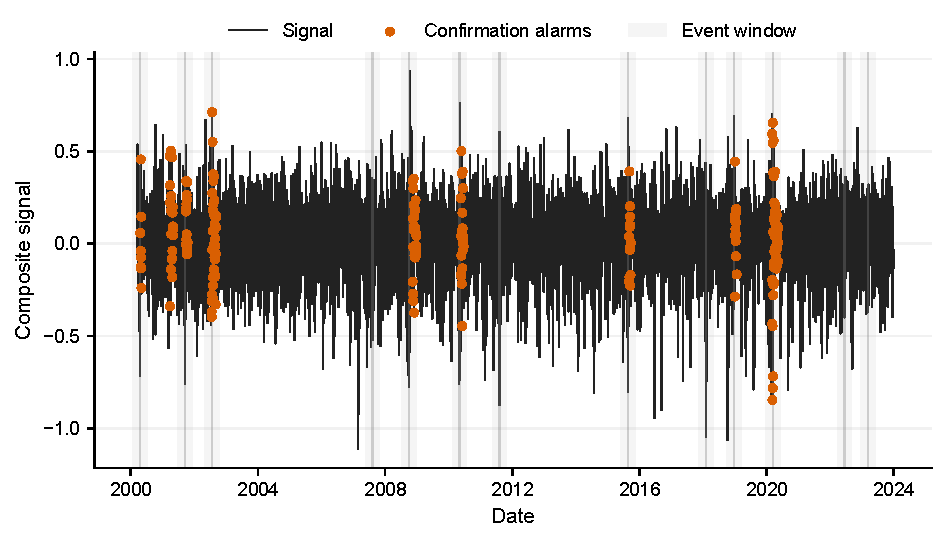
\includegraphics[width=\textwidth]{Fig1.pdf}
\caption{SPY timeline with the fixed event windows and the alarms raised by the confirmation rule.}
\label{fig:spy_timeline}
\end{figure*}

\subsection{Comparison with a published volatility index}
\label{sec:vix}
The volatility percentile trigger and the confirmation rule are both defined in this paper, so the reversal between them could be a property of those two rules rather than of the protocol. To separate the two possibilities, we replace the volatility percentile trigger with the Cboe Volatility Index and leave everything else unchanged, including the instability condition. Table~\ref{tab:vix} reports the result on the SPY panel.

The VIX trigger detects 10 of 13 events, the same number as the volatility trigger, and alarms earlier, at $-4.4$ trading days against $-1.2$. The two reach that count on different events: VIX detects Volmageddon, which both study detectors miss, and misses the dot-com selloff, where implied volatility was already high throughout the calibration period.

Adding the same instability condition raises precision from 0.596 to 0.947, lowers the false positive rate from 0.048 to 0.002, and reduces alarm days outside every window from 214 to 9. Detection falls from 10 events to 7. The crossover ratio against the unconfirmed VIX trigger is 0.022, against 0.021 for the pair built here. Because the instability condition is held fixed, this isolates the first condition: the reversal does not depend on the volatility trigger, and the confirmation layer is not tested by it.

\begin{table*}[t]
\centering
\caption{Comparison against a published volatility index on the SPY event panel, with the same calibration, smoothing, thresholds, and event windows. $A_{\mathrm{out}}$ counts alarm days outside every event window; $r^{*}$ is the crossover of Equation~\eqref{eq:crossover} against the VIX trigger at $c_{\mathrm{D}}=0.05$.}
\label{tab:vix}
\begin{tabular}{lrrrrrrrr}
\toprule
Method & Precision & Recall & F1 & FPR & Events & Delay & $A_{\mathrm{out}}$ & $r^{*}$\\
\midrule
VIX percentile & 0.596 & 0.206 & 0.306 & 0.048 & 10/13 & -4.4 & 214 & \\
Volatility percentile & 0.640 & 0.225 & 0.333 & 0.044 & 10/13 & -1.2 & 195 & 0.061\\
Confirmation ($W=10$) & 0.886 & 0.122 & 0.214 & 0.005 & 8/13 & 6.8 & 24 & 0.025\\
VIX + instability & 0.947 & 0.106 & 0.190 & 0.002 & 7/13 & 3.7 & 9 & 0.022\\
\bottomrule
\end{tabular}
\end{table*}

\subsection{Multi-asset results}
The protocol is applied unchanged to the four remaining assets. Table~\ref{tab:multiasset_pointwise} and Figure~\ref{fig:multiasset_tradeoff} give the day-level results for all five. The same pattern holds on every asset: the confirmation rule has the lower false positive rate, and it also has the lower recall and the lower F1. The size of the difference varies. On QQQ the false positive rate falls from 0.039 to 0.006 and F1 falls from 0.280 to 0.139. On IWM the false positive rate falls from 0.056 to 0.028 and F1 falls from 0.272 to 0.159. HYG and TLT show the same pattern. They differ in delay, and on TLT in precision as well: on HYG the confirmation rule alarms earlier than the volatility trigger and on TLT it alarms later, and TLT is the only asset on which the confirmation rule has the lower precision, 0.367 against 0.507.

\begin{table*}[t]
\centering
\caption{Day-level results for the volatility trigger and the confirmation rule on all five assets.}
\label{tab:multiasset_pointwise}
\scriptsize
\begin{tabular}{llrrrrrr}
\toprule
Asset & Method & Precision & Recall & F1 & FPR & Mean delay & Align. err.\\
\midrule
SPY & Volatility & 0.640 & 0.225 & 0.333 & 0.044 & -1.2 & 3.6\\
SPY & Confirmation & 0.886 & 0.122 & 0.214 & 0.005 & 6.8 & 8.3\\
QQQ & Volatility & 0.616 & 0.181 & 0.280 & 0.039 & -19.3 & 3.2\\
QQQ & Confirmation & 0.812 & 0.076 & 0.139 & 0.006 & 10.4 & 15.2\\
IWM & Volatility & 0.529 & 0.183 & 0.272 & 0.056 & -0.3 & 4.4\\
IWM & Confirmation & 0.536 & 0.093 & 0.159 & 0.028 & 14.2 & 16.2\\
HYG & Volatility & 0.501 & 0.163 & 0.246 & 0.064 & 0.2 & 2.2\\
HYG & Confirmation & 0.650 & 0.110 & 0.188 & 0.024 & -1.0 & 2.3\\
TLT & Volatility & 0.507 & 0.281 & 0.362 & 0.085 & -25.3 & 4.7\\
TLT & Confirmation & 0.367 & 0.094 & 0.150 & 0.051 & -4.8 & 23.5\\
\bottomrule
\end{tabular}
\end{table*}

\begin{figure*}[t]
\centering
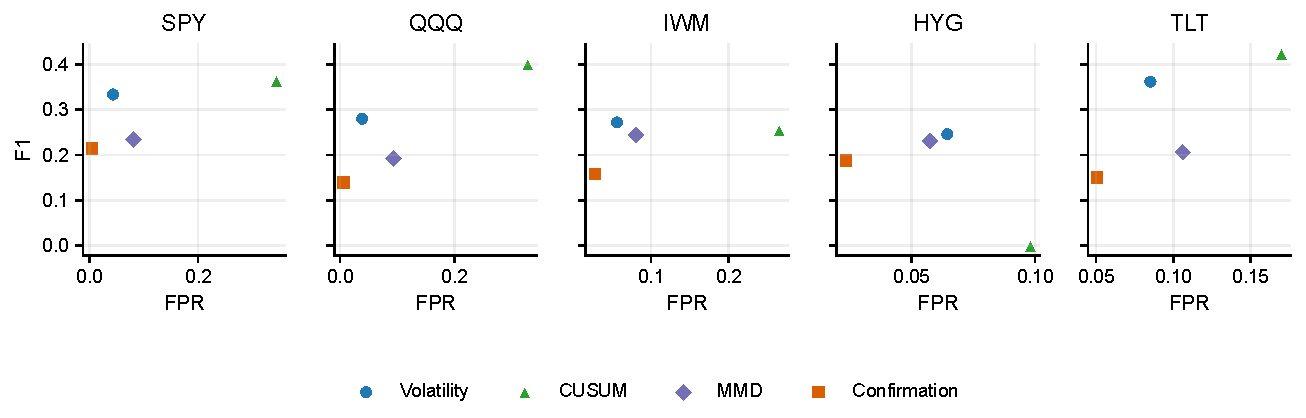
\includegraphics[width=\textwidth]{Fig2.pdf}
\caption{False positive rate against F1 on all five assets under the same protocol, with no per-asset tuning.}
\label{fig:multiasset_tradeoff}
\end{figure*}

\subsection{Event-level results}
Day-level recall and the false positive rate do not record whether an event received any alarm at all. Table~\ref{tab:spy_event_level} and Figure~\ref{fig:event_level_delay} give the event-level comparison on SPY. The confirmation rule detects 8 of the 13 events and the volatility trigger detects 10. The confirmation rule misses the U.S. downgrade and the 2022 inflation selloff, both of which the volatility trigger detects. Neither detects the quant crisis, Volmageddon, or the 2023 bank stress episode. On the eight events both detect, the confirmation rule never covers a larger fraction of the window, equalling the volatility trigger on four of them and covering less on the other four, and its first alarm is never earlier. The largest difference is the Lehman episode, where the volatility trigger alarms 7 trading days before the event date and the confirmation rule alarms 33 days after it.

The thresholds are calibrated on the first 70 per cent of the SPY series, which ends in 2016. Eight events fall inside that period and five fall after it. Of the eight inside, the volatility trigger detects seven and the confirmation rule detects six. Of the five after it, the volatility trigger detects three and the confirmation rule detects two. Both detect fewer events after the calibration period, and the volatility trigger detects more events than the confirmation rule in both groups.

\begin{table*}[t]
\centering
\caption{Event-level detection, first-alarm delay, and window coverage on SPY.}
\label{tab:spy_event_level}
\scriptsize
\begin{tabular}{llrrrrrr}
\toprule
Event & Severity & Vol. det. & Conf. det. & Vol. delay & Conf. delay & Vol. cov. & Conf. cov.\\
\midrule
Dot-com selloff & high & 1 & 1 & 4 & 4 & 0.241 & 0.096\\
September 11 reopening & critical & 1 & 1 & 6 & 6 & 0.132 & 0.124\\
WorldCom selloff & critical & 1 & 1 & -8 & -4 & 0.446 & 0.306\\
Quant crisis & medium & 0 & 0 & NA & NA & 0.000 & 0.000\\
Lehman crisis & critical & 1 & 1 & -7 & 33 & 0.562 & 0.231\\
Flash crash & high & 1 & 1 & 11 & 11 & 0.174 & 0.174\\
U.S. downgrade & critical & 1 & 0 & 2 & NA & 0.405 & 0.000\\
China devaluation & medium & 1 & 1 & 8 & 8 & 0.116 & 0.116\\
Volmageddon & medium & 0 & 0 & NA & NA & 0.000 & 0.000\\
Q4 2018 selloff & high & 1 & 1 & 4 & 4 & 0.124 & 0.124\\
COVID crash & critical & 1 & 1 & -8 & -8 & 0.405 & 0.405\\
Inflation selloff & high & 1 & 0 & -24 & NA & 0.331 & 0.000\\
Bank stress & medium & 0 & 0 & NA & NA & 0.000 & 0.000\\
\bottomrule
\end{tabular}
\end{table*}

\subsubsection{Which component fails}
\label{sec:mechanism}
Table~\ref{tab:mechanism} splits each event window into volatility alarm days, instability alarm days, and the highest smoothed $z_{\mathrm{MMD}}$ reached inside it. Four observations follow from it.
\begin{itemize}
\item The instability condition never held on the two missed events. It held on 1 of the 121 window days for the U.S. downgrade and on 2 for the inflation selloff, against 10 to 49 days, mean 28.0, across the eight detected events.
\item The volatility condition is not responsible. It held on 49 and 40 days in those two windows.
\item The kernel statistic is. Its peak reaches 0.96 and 1.84 in those windows, against a mean of 3.38 across detected events.
\item The cause is the composite signal. Because $x_t$ is close to a return divided by the standard deviation of the previous 50 days, a rise in volatility that those 50 days absorb leaves the distribution of $x_t$ unchanged. Measured against the 120 trading days before each window, the spread of raw volatility rises by a factor of 3.03 across the seven detected events with a full preceding window, while the spread of $x_t$ rises by 1.29. For the U.S. downgrade the two factors are 3.26 and 1.24; for the inflation selloff they are 1.11 and 0.85.
\end{itemize}
Two other explanations do not fit. The missed events are not the slower ones: their peak-to-trough spans average 13.2 trading days against 22.5 for detected events. They are not simply the smaller ones either: mean severity is 0.110 for missed events against 0.196 for detected ones, but the U.S. downgrade has a severity of 0.166 and a worst day of 6.73 per cent, larger than six of the eight detected events, and is still missed. The two detectors therefore measure different quantities. One reads the level of volatility; the other reads how far returns move relative to the trailing scale.

\begin{table*}[t]
\centering
\caption{Component counts for each SPY event window ($\pm60$ trading days, at most 121 days per window; the dot-com window is clamped to 83 days because it begins at the start of the processed series). Alarm days are counted inside the window; peak $z_{\mathrm{MMD}}$ is the highest smoothed standardized MMD reached there.}
\label{tab:mechanism}
\scriptsize
\begin{tabular}{lrrrrr}
\toprule
Event & Vol. det. & Conf. det. & Vol. alarm days & Instab. alarm days & Peak $z_{\mathrm{MMD}}$\\
\midrule
Dot-com selloff & 1 & 1 & 20 & 21 & 4.39\\
September 11 reopening & 1 & 1 & 16 & 20 & 1.79\\
WorldCom selloff & 1 & 1 & 54 & 17 & 2.14\\
Quant crisis & 0 & 0 & 0 & 24 & 2.71\\
Lehman crisis & 1 & 1 & 68 & 10 & 2.15\\
Flash crash & 1 & 1 & 21 & 49 & 4.88\\
U.S. downgrade & 1 & 0 & 49 & 1 & 0.96\\
China devaluation & 1 & 1 & 14 & 44 & 2.44\\
Volmageddon & 0 & 0 & 0 & 7 & 1.62\\
Q4 2018 selloff & 1 & 1 & 15 & 17 & 2.65\\
COVID crash & 1 & 1 & 49 & 46 & 6.56\\
Inflation selloff & 1 & 0 & 40 & 2 & 1.84\\
Bank stress & 0 & 0 & 0 & 0 & 0.14\\
\bottomrule
\end{tabular}
\end{table*}

\subsubsection{Synthetic test of the mechanism}
\label{sec:mechtest}
The explanation above rests on two events, so the same mechanism is tested on generated data, where the episodes can be constructed. We generate a Gaussian return series and apply the same preprocessing, calibration, thresholds, and confirmation rule to it. The series contains two episodes that reach the same peak volatility, three times the baseline level. Episode A reaches that peak in one day and holds it for 60 days. Episode B reaches the same peak and returns to baseline along a symmetric 300-day triangle, slowly enough for the trailing 50-day scale to follow it. A third abrupt episode is placed inside the calibration period.

The volatility trigger alarms in both episodes: on 54 of the 60 days in A and on 254 of the 300 days in B. The confirmation condition separates them. Using MMD alone, it alarms on 36 of the 60 days in A, 60 per cent, and on 9 of the 300 days in B, 3 per cent. The peak smoothed $z_{\mathrm{MMD}}$ is 4.95 in A and 1.79 in B. A 90th-percentile threshold alarms on 10 per cent of calibration days by construction, so A is six times that rate and B is below it. The full instability score gives 57 per cent in A and 7 per cent in B, and the alarms in B come from the two-sided $\kappa$ term rather than from the kernel statistic. An episode that the trailing scale absorbs is therefore not registered by the confirmation layer, even at three times the baseline volatility.

\begin{figure*}[t]
\centering
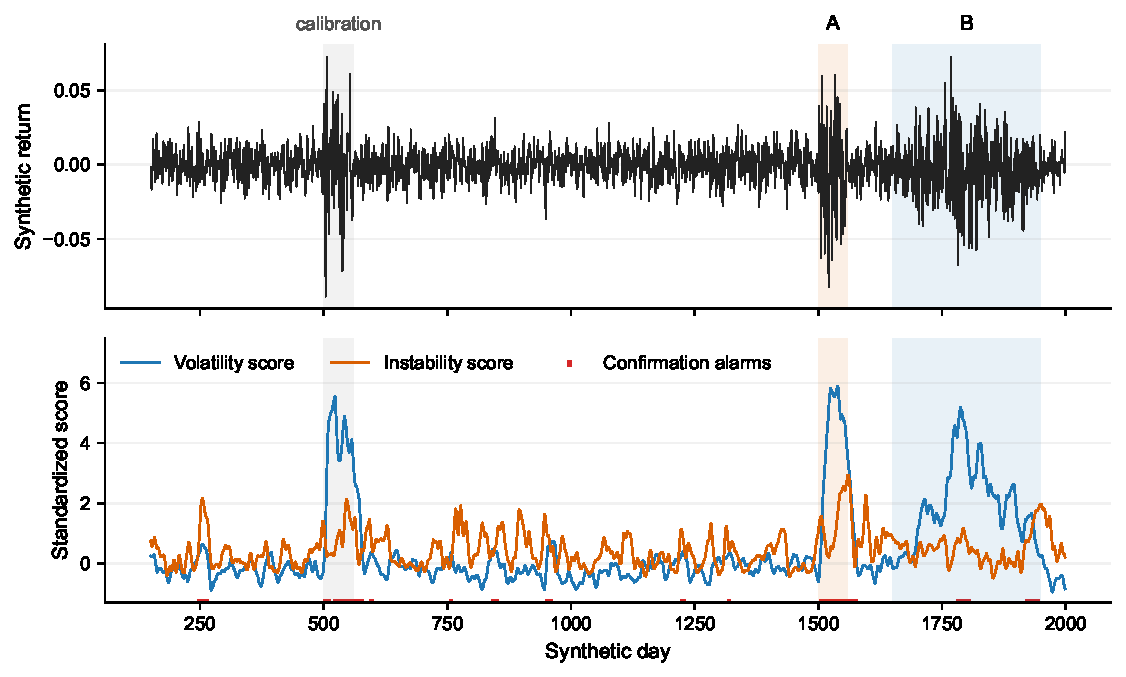
\includegraphics[width=0.9\textwidth]{Fig3.pdf}
\caption{Synthetic test of the scale mechanism. Top: a Gaussian return series with an abrupt volatility break (A), an absorbed triangle ramp (B) of the same peak volatility, and the abrupt calibration episode. Bottom: standardized volatility and instability scores with the resulting alarms. The volatility score rises in both episodes; the instability score responds only to the abrupt break.}
\label{fig:mechtest}
\end{figure*}

\subsubsection{Multi-asset event-level results}
Table~\ref{tab:multiasset_event_level} gives the event-level results for all five assets. The volatility trigger detects more events on each one: 0.769 against 0.615 on SPY, 0.462 against 0.385 on QQQ, 0.538 against 0.385 on IWM, 0.385 against 0.231 on HYG, and 0.538 against 0.308 on TLT. Mean coverage is lower for the confirmation rule on every asset, and its median first alarm is later on every asset except HYG.

These rates use all 13 events as the denominator, but the processed series begin later than the panel does: IWM in August 2000, TLT in October 2002, and HYG in June 2007, each 50 trading days after the asset's inception because of the warm-up. Some events therefore precede the series. Each such event is mapped to the asset's first available date, which gives one empty window for IWM and three each for HYG and TLT. Neither detector alarms in an empty window, so the rates for HYG and TLT are lowered by construction. Over the events each asset can observe, the counts are 7 against 5 of 12 for IWM, 5 against 3 of 10 for HYG, and 7 against 4 of 10 for TLT, with the volatility trigger first in each pair. The comparison within an asset is unaffected, since both detectors face the same events. The cost results are also unaffected, because the difference in missed events entering Equation~\eqref{eq:crossover} is the same with or without the empty windows.

\begin{table*}[t]
\centering
\caption{Event-level detection rate, median first-alarm delay, and mean window coverage. All rates use the 13-event panel as denominator; rates over each asset's observable events are given in the text.}
\label{tab:multiasset_event_level}
\scriptsize
\begin{tabular}{llrrr}
\toprule
Asset & Method & Detect. rate & Med. delay & Mean cov.\\
\midrule
SPY & Vol. & 0.769 & 3.0 & 0.226\\
SPY & Confirm. & 0.615 & 5.0 & 0.121\\
QQQ & Vol. & 0.462 & -11.5 & 0.198\\
QQQ & Confirm. & 0.385 & 2.0 & 0.086\\
IWM & Vol. & 0.538 & 1.0 & 0.176\\
IWM & Confirm. & 0.385 & 5.0 & 0.090\\
HYG & Vol. & 0.385 & 2.0 & 0.123\\
HYG & Confirm. & 0.231 & -3.0 & 0.083\\
TLT & Vol. & 0.538 & -4.0 & 0.227\\
TLT & Confirm. & 0.308 & -2.5 & 0.076\\
\bottomrule
\end{tabular}
\end{table*}

\subsubsection{Detection by severity}
\label{sec:severity_detection}
Table~\ref{tab:event_level_severity} groups events by severity, averaging each rate over the five assets. The confirmation rule detects 0.680 of critical events, 0.300 of high, and 0.100 of medium, against 0.840, 0.550, and 0.150 for the volatility trigger. Its detection falls off more steeply, which is what a rule keyed to scale contrast produces. With 13 events in three groups these are descriptive figures.

\begin{table*}[t]
\centering
\caption{Event-level results by severity tercile. The terciles are the realized-drawdown groups of the SPY panel; each figure is the mean over the five assets.}
\label{tab:event_level_severity}
\scriptsize
\begin{tabular}{llrrr}
\toprule
Severity & Method & Detect. rate & Med. delay & Mean cov.\\
\midrule
Critical & Vol. & 0.840 & -2.6 & 0.317\\
Critical & Confirm. & 0.680 & 2.0 & 0.176\\
High & Vol. & 0.550 & -8.9 & 0.175\\
High & Confirm. & 0.300 & -1.3 & 0.066\\
Medium & Vol. & 0.150 & -26.0 & 0.046\\
Medium & Confirm. & 0.100 & -26.0 & 0.011\\
\bottomrule
\end{tabular}
\end{table*}

\begin{figure*}[t]
\centering
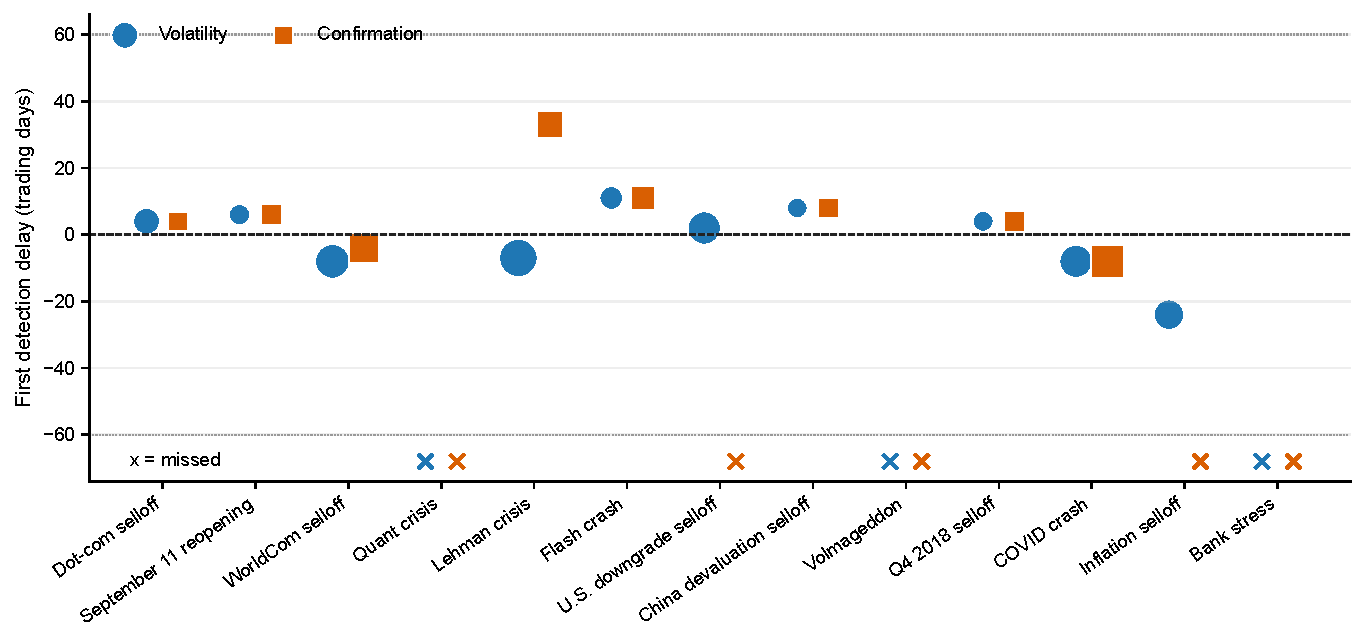
\includegraphics[width=0.95\textwidth]{Fig4.pdf}
\caption{First-alarm delay and window coverage for each SPY event, with missed events marked.}
\label{fig:event_level_delay}
\end{figure*}

\subsection{Costs}
\label{sec:cost}
Table~\ref{tab:cost} and Figure~\ref{fig:cost} give the day-level cost with $c_{\mathrm{FN}}=1$. The confirmation rule has the lower cost at every ratio tested. At $c_{\mathrm{FP}}/c_{\mathrm{FN}}=1$ the two costs are 1372 and 1384, and the difference widens as false positives are made more expensive, reaching 2548 against 10939 at a ratio of 50. The 13 event windows cover 1535 of the 5987 trading days in the SPY sample: no two windows overlap, so the total is 13 windows of 121 days less the 38 days by which the dot-com window is clamped at the start of the series. Most days therefore lie outside every window, and a false positive is counted far more often than a false negative. A detector that alarms on fewer of those outside days therefore has the lower cost under this model, even when it has the lower recall, the lower detection rate, and the later first alarm.

Table~\ref{tab:event_cost} gives the event-level cost with $c_{\mathrm{ME}}=1$ and $c_{\mathrm{D}}=0.05$. At $c_{\mathrm{FA}}/c_{\mathrm{ME}}=0.01$ the volatility trigger costs 6.70 and the confirmation rule 8.54, because the volatility trigger misses 3 events rather than 5 and carries a smaller delay term, $D_+=35$ against 66. At 0.05 and above the confirmation rule costs less, because it alarms on 24 days outside the windows and the volatility trigger alarms on 195.

\begin{table}[t]
\centering
\caption{Day-level cost comparison with $c_{\mathrm{FN}}=1$.}
\label{tab:cost}
\scriptsize
\begin{tabular}{rrrr}
\toprule
$c_{\mathrm{FP}}/c_{\mathrm{FN}}$ & Vol. cost & Confirm. cost & Lower cost\\
\midrule
1 & 1384 & 1372 & Confirmation\\
2 & 1579 & 1396 & Confirmation\\
5 & 2164 & 1468 & Confirmation\\
10 & 3139 & 1588 & Confirmation\\
20 & 5089 & 1828 & Confirmation\\
50 & 10939 & 2548 & Confirmation\\
\bottomrule
\end{tabular}
\end{table}

\begin{table*}[t]
\centering
\caption{SPY event-level cost comparison with $c_{\mathrm{ME}}=1$ and $c_{\mathrm{D}}=0.05$.}
\label{tab:event_cost}
\scriptsize
\begin{tabular}{lrrrr}
\toprule
$c_{\mathrm{FA}}/c_{\mathrm{ME}}$ & Vol. cost & Confirm. cost & Vol. missed & Confirm. missed\\
\midrule
0.01 & 6.70 & 8.54 & 3 & 5\\
0.05 & 14.50 & 9.50 & 3 & 5\\
0.10 & 24.25 & 10.70 & 3 & 5\\
0.25 & 53.50 & 14.30 & 3 & 5\\
0.50 & 102.25 & 20.30 & 3 & 5\\
1.00 & 199.75 & 32.30 & 3 & 5\\
\bottomrule
\end{tabular}
\end{table*}

\subsubsection{Crossover ratio}
Equation~\eqref{eq:eventcost} is linear in $c_{\mathrm{FA}}$, so the two costs can be set equal and solved for the value of $c_{\mathrm{FA}}/c_{\mathrm{ME}}$ at which the two detectors cost the same:
\begin{equation}
\label{eq:crossover}
r^{*}=\frac{(M_{\mathrm{conf}}-M_{\mathrm{vol}})+c_{\mathrm{D}}\,(D_{+}^{\mathrm{conf}}-D_{+}^{\mathrm{vol}})}{A_{\mathrm{out}}^{\mathrm{vol}}-A_{\mathrm{out}}^{\mathrm{conf}}}.
\end{equation}
Here $M$ is the number of missed events, $D_+$ is the sum of the positive first-alarm delays over detected events, and $A_{\mathrm{out}}$ is the number of alarm days outside every event window, each with the subscript "conf" for the confirmation rule and "vol" for the volatility trigger. The numerator is therefore the extra missed events and extra delay of the confirmation rule, and the denominator is the alarm days it saves. Since the confirmation rule alarms on fewer days outside the windows, the denominator is positive, and the volatility trigger has the lower cost when $c_{\mathrm{FA}}/c_{\mathrm{ME}}$ is below $r^{*}$ and the confirmation rule when it is above.

For SPY at $c_{\mathrm{D}}=0.05$,
\begin{equation}
r^{*}=\frac{(5-3)+0.05\,(66-35)}{195-24}=\frac{3.55}{171}=0.021 .
\end{equation}
The volatility trigger therefore has the lower cost on SPY only when one alarm day outside the windows costs less than 0.021 of a missed episode, that is, when a missed episode is worth more than 48 such alarm days. The tested values cross this point between 0.01 and 0.05.

Table~\ref{tab:crossover} gives $r^{*}$ for the five assets and the three delay penalties. All values lie between 0.007 and 0.059. On four of the five assets $r^{*}$ rises as $c_{\mathrm{D}}$ rises, because the confirmation rule alarms later there and so carries more of the delay penalty. On HYG $r^{*}$ falls, from 0.016 to 0.013, because HYG is the one asset on which the confirmation rule alarms earlier than the volatility trigger.


\begin{table}[t]
\centering
\caption{Crossover ratio $r^{*}=c_{\mathrm{FA}}/c_{\mathrm{ME}}$ from Equation~\eqref{eq:crossover}. Below $r^{*}$ the volatility trigger has the lower cost; above it the confirmation rule does.}
\label{tab:crossover}
\scriptsize
\begin{tabular}{lrrr}
\toprule
Asset & $c_{\mathrm{D}}=0$ & $c_{\mathrm{D}}=0.05$ & $c_{\mathrm{D}}=0.1$\\
\midrule
SPY & 0.012 & 0.021 & 0.030\\
QQQ & 0.007 & 0.027 & 0.047\\
IWM & 0.016 & 0.038 & 0.059\\
HYG & 0.016 & 0.015 & 0.013\\
TLT & 0.021 & 0.034 & 0.047\\
\bottomrule
\end{tabular}
\end{table}

\begin{figure*}[t]
\centering
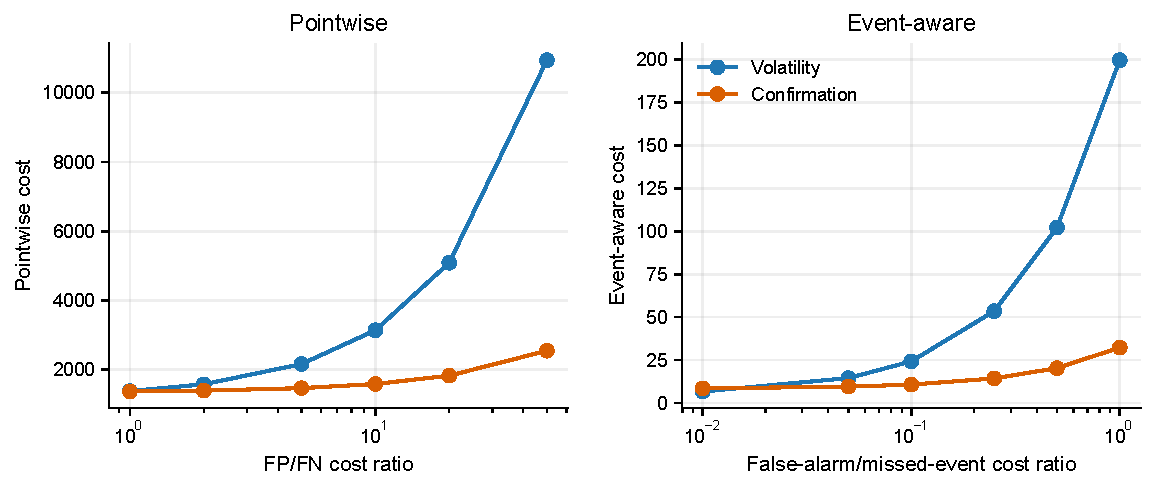
\includegraphics[width=0.7\textwidth]{Fig5.pdf}
\caption{SPY cost comparison under the day-level and event-level cost models.}
\label{fig:cost}
\end{figure*}

\subsection{Sensitivity analyses}
\subsubsection{Event-window width}
Table~\ref{tab:eventwindow} and Figure~\ref{fig:eventwindow} repeat the evaluation at $\pm20$, $\pm30$, $\pm45$, and $\pm60$ trading days. The confirmation rule has the higher precision and the lower false positive rate at every width, and the lower recall and F1. The precision gap grows with width, from 0.155 at $\pm20$ to 0.247 at $\pm60$, since wider windows admit more of the volatility trigger's alarms; the gap in false positive rate narrows slightly, from 0.043 to 0.038.

\begin{table*}[t]
\centering
\caption{Day-level precision, recall, F1, and false positive rate at four event-window widths.}
\label{tab:eventwindow}
\scriptsize
\begin{tabular}{llrrrr}
\toprule
Window & Method & Prec. & Recall & F1 & FPR\\
\midrule
$\pm20$ & Vol. & 0.390 & 0.396 & 0.393 & 0.061\\
$\pm20$ & Confirm. & 0.545 & 0.216 & 0.309 & 0.018\\
$\pm30$ & Vol. & 0.499 & 0.344 & 0.407 & 0.052\\
$\pm30$ & Confirm. & 0.692 & 0.186 & 0.293 & 0.012\\
$\pm45$ & Vol. & 0.571 & 0.266 & 0.363 & 0.048\\
$\pm45$ & Confirm. & 0.815 & 0.148 & 0.251 & 0.008\\
$\pm60$ & Vol. & 0.640 & 0.225 & 0.333 & 0.044\\
$\pm60$ & Confirm. & 0.886 & 0.122 & 0.214 & 0.005\\
\bottomrule
\end{tabular}
\end{table*}

\begin{figure*}[t]
\centering
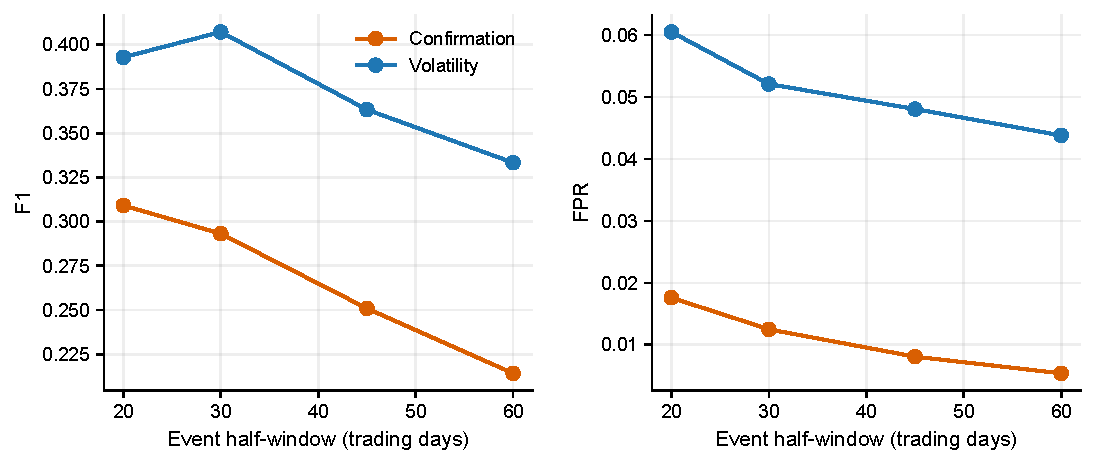
\includegraphics[width=0.60\textwidth]{Fig6.pdf}
\caption{Results at $\pm20$, $\pm30$, $\pm45$, and $\pm60$ trading-day event windows.}
\label{fig:eventwindow}
\end{figure*}

\subsubsection{Composite weights}
\label{sec:weights}
Table~\ref{tab:weights} re-runs the pipeline under ten weightings, recomputing $x_t$, MMD, $\kappa$, the instability score, and the confirmation rule each time. The volatility trigger is unchanged, since it reads $\sigma_t$ directly. Across the ten weightings, F1 stays within $[0.210,0.235]$ and the false positive rate within $[0.005,0.009]$. The confirmation rule detects 8 of the 13 events under nine weightings and 7 under the tenth. The volatility trigger has an F1 of 0.333, a false positive rate of 0.044, and 10 detected events, and no weighting brings the confirmation rule close to those three values.

Six of the ten weightings give identical results: the default, the equal weighting, the reversed weighting, $(0.4,0.4,0.2)$, $(0.5,0.2,0.3)$, and $z$-score only. This follows from the scale of the three terms. The standard deviation of $z_t$ is two orders of magnitude above that of the other two terms, so moving weight between them leaves $x_t$ effectively unchanged, and the kernel statistic reads the same series. The four remaining weightings differ. Two of them keep $z_t$ but change its share: $(0.6,0.2,0.2)$ lowers precision to 0.882 and raises the false positive rate to 0.006, and $(0.2,0.6,0.2)$ raises precision to 0.900 and F1 to 0.235 and moves the mean first alarm to 4.4 trading days after the event. The largest departures come from the two weightings that remove $z_t$ altogether. With volatility alone, the confirmation rule detects 7 events instead of 8 and its false positive rate rises to 0.009. With returns alone, its mean first alarm is 0.8 trading days after the event, the earliest in the table, and its precision falls to 0.845.

\begin{table*}[t]
\centering
\caption{Composite weight ablation. Each row recomputes $x_t$, the MMD and $\kappa$ components, and the confirmation rule. Events are counted out of 13.}
\label{tab:weights}
\scriptsize
\begin{tabular}{lrrrrrr}
\toprule
$(w_r,w_\sigma,w_z)$ & Prec. & Recall & F1 & FPR & Delay & Events\\
\midrule
$(0.5,0.3,0.2)$ default & 0.886 & 0.122 & 0.214 & 0.005 & 6.8 & 8\\
$(1/3,1/3,1/3)$ equal & 0.886 & 0.122 & 0.214 & 0.005 & 6.8 & 8\\
$(0.2,0.3,0.5)$ reversed & 0.886 & 0.122 & 0.214 & 0.005 & 6.8 & 8\\
$(0.6,0.2,0.2)$ & 0.882 & 0.122 & 0.214 & 0.006 & 6.8 & 8\\
$(0.4,0.4,0.2)$ & 0.886 & 0.122 & 0.214 & 0.005 & 6.8 & 8\\
$(0.5,0.2,0.3)$ & 0.886 & 0.122 & 0.214 & 0.005 & 6.8 & 8\\
$(0.2,0.6,0.2)$ & 0.900 & 0.135 & 0.235 & 0.005 & 4.4 & 8\\
$(1,0,0)$ returns only & 0.845 & 0.131 & 0.227 & 0.008 & 0.8 & 8\\
$(0,1,0)$ volatility only & 0.815 & 0.121 & 0.210 & 0.009 & 1.4 & 7\\
$(0,0,1)$ $z$-score only & 0.886 & 0.122 & 0.214 & 0.005 & 6.8 & 8\\
\bottomrule
\end{tabular}
\end{table*}

\subsubsection{Sign of $\kappa$}
\label{sec:kappasign}
The instability score uses $|z_\kappa|$, so it responds to $\kappa$ moving away from its calibration mean in either direction. Table~\ref{tab:kappasign} compares this with the two versions that respond in one direction only: $\max(-z_\kappa,0)$, which responds only when $\kappa$ falls below its mean, and $\max(+z_\kappa,0)$, which responds only when it rises above. Theory on approaching regime shifts predicts the first of these. Using it, the confirmation rule detects 7 events instead of 8 and its F1 falls to 0.202. Using the second, it also detects 7 events, its F1 rises to 0.242, and its mean first alarm moves to 1.6 trading days after the event. The three F1 values, 0.202 to 0.242, span a slightly wider range than the weight ablation's $[0.210,0.235]$.

\begin{table*}[t]
\centering
\caption{Ablation on the persistence statistic. The low-$\kappa$ variant is the direction predicted by theory on approaching regime shifts.}
\label{tab:kappasign}
\scriptsize
\begin{tabular}{lrrrrrr}
\toprule
Confirmation term & Prec. & Recall & F1 & FPR & Delay & Events\\
\midrule
$|z_\kappa|$ two-sided (default) & 0.886 & 0.122 & 0.214 & 0.005 & 6.8 & 8\\
$\max(-z_\kappa,0)$ low $\kappa$ & 0.875 & 0.114 & 0.202 & 0.006 & 6.7 & 7\\
$\max(+z_\kappa,0)$ high $\kappa$ & 0.874 & 0.141 & 0.242 & 0.007 & 1.6 & 7\\
\bottomrule
\end{tabular}
\end{table*}

\subsubsection{Causal confirmation}
\label{sec:causal}
The confirmation rule uses days after $t$ in two places: the window $[t-W,t+W]$, which extends $W$ days past $t$, and the MMD statistic, whose second sample is the 30 days from $t$ to $t+29$. Table~\ref{tab:causal} removes these two sources of future data, first separately and then together.

Replacing the window with $[t-W,t]$ leaves detection at 8 of 13 events, raises precision to 0.917, and reduces alarm days outside the windows from 24 to 14, while recall falls and the mean first alarm moves to 10.8 trading days after the event. Individual events are confirmed later: WorldCom moves from 4 days before the event to 6 days after, the Flash Crash from 11 days after to 21, and Lehman from 33 days after to 43. The crossover ratio becomes 0.027, and every conclusion above holds for this variant.

Lagging the MMD component by the length of its second sample removes the remaining use of future data. Detection then falls to 4 of 13 events at $W=10$. Widening the window to $W=40$ restores detection to 7 of 13 but raises alarm days outside the windows from 24 to 105, giving back 81 of the 171-day gap to the volatility trigger's 195. Most of the selectivity of the confirmation layer therefore comes from the MMD second sample rather than from the confirmation window. The crossover ratio rises across these variants to at most 0.058.

\begin{table*}[t]
\centering
\caption{Removing the use of future data on SPY. Trailing variants replace $[t-W,t+W]$ with $[t-W,t]$; causal variants also lag the MMD component by its 30-day second sample, so no input uses future data. $r^{*}$ is the crossover of Equation~\eqref{eq:crossover} at $c_{\mathrm{D}}=0.05$.}
\label{tab:causal}
\scriptsize
\begin{tabular}{lrrrrrrrr}
\toprule
Variant & Prec. & Recall & F1 & FPR & Events & Delay & $A_{\mathrm{out}}$ & $r^{*}$\\
\midrule
Symmetric $W=10$ (default) & 0.886 & 0.122 & 0.214 & 0.005 & 8/13 & 6.8 & 24 & 0.021\\
Trailing $W=10$ & 0.917 & 0.100 & 0.181 & 0.003 & 8/13 & 10.8 & 14 & 0.027\\
Trailing $W=20$ & 0.838 & 0.115 & 0.202 & 0.008 & 8/13 & 9.5 & 34 & 0.028\\
Causal, $W=10$ & 0.659 & 0.058 & 0.107 & 0.010 & 4/13 & 15.8 & 46 & 0.051\\
Causal, $W=40$ & 0.568 & 0.090 & 0.155 & 0.024 & 7/13 & 10.3 & 105 & 0.058\\
Volatility (reference) & 0.640 & 0.225 & 0.333 & 0.044 & 10/13 & -1.2 & 195 & \\
\bottomrule
\end{tabular}
\end{table*}

\subsubsection{Severity, components, and confirmation window}
Grouping the days by the severity of the event whose window they fall in gives the same ordering as the event-level results in the two higher terciles. In the highest tercile, F1 is 0.412 for the volatility trigger and 0.316 for the confirmation rule, and the false positive rate is 0.057 against 0.015. In the middle tercile, F1 is 0.195 against 0.134 and the false positive rate 0.080 against 0.030. In the lowest tercile both values are near zero, 0.027 against 0.040, and the false positive rate is 0.096 against 0.036, on 14 true positives for each detector, too few for the F1 ordering to be meaningful.

Replacing the instability score with MMD alone as the confirmation signal gives an F1 of 0.219 against 0.214 for the default, with a false positive rate of 0.011 against 0.005. Figure~\ref{fig:window_sensitivity} shows how the results change with the width $W$ of the confirmation window. F1 rises to 0.291 at $W=60$, so the default $W=10$ does not give the highest F1, but the false positive rate rises to 0.031 at that width. These variants use the window $[t-W,t+W]$ and so describe the rule that reads days after the alarm.

\begin{figure*}[t]
\centering
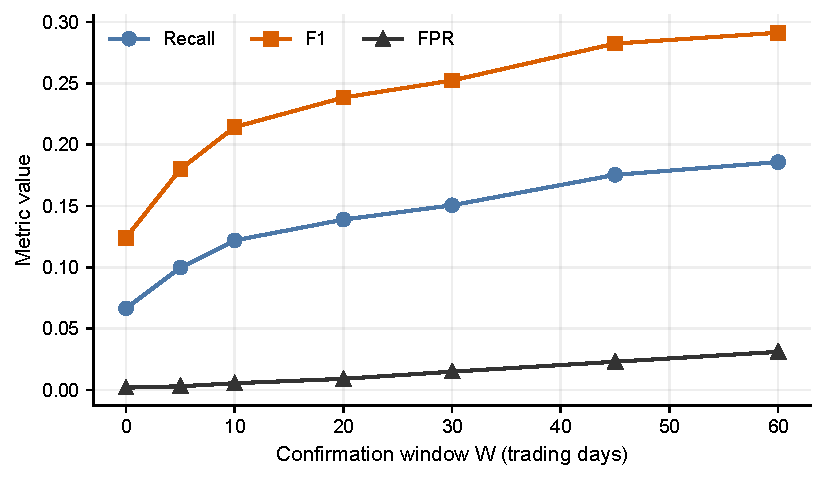
\includegraphics[width=0.50\textwidth]{Fig7.pdf}
\caption{Effect of the confirmation window width $W$ on F1 and the false positive rate.}
\label{fig:window_sensitivity}
\end{figure*}

\subsection{Confidence intervals}
\label{sec:bootstrap}
Each difference below is the value for the confirmation rule less the value for the volatility trigger, so a negative value means the confirmation rule is lower. The event bootstrap gives a difference in F1 of $-0.091$ with interval $[-0.166,0.005]$ and a difference in false positive rate of $-0.045$ with interval $[-0.058,-0.035]$. The block bootstrap gives $-0.120$ with $[-0.203,-0.047]$ and $-0.039$ with $[-0.062,-0.019]$. The difference in false positive rate is negative in all 2000 resamples under both schemes. The difference in F1 is negative in all 2000 block resamples and in 97.3 per cent of event resamples, and its event interval includes zero. Figure~\ref{fig:bootstrap_violin} shows the distributions. Neither scheme goes outside this panel: the event scheme resamples its 13 events and the block scheme resamples blocks of the daily series scored against them. The intervals therefore measure variability within the panel and say nothing about events outside it.

\begin{figure*}[t]
\centering
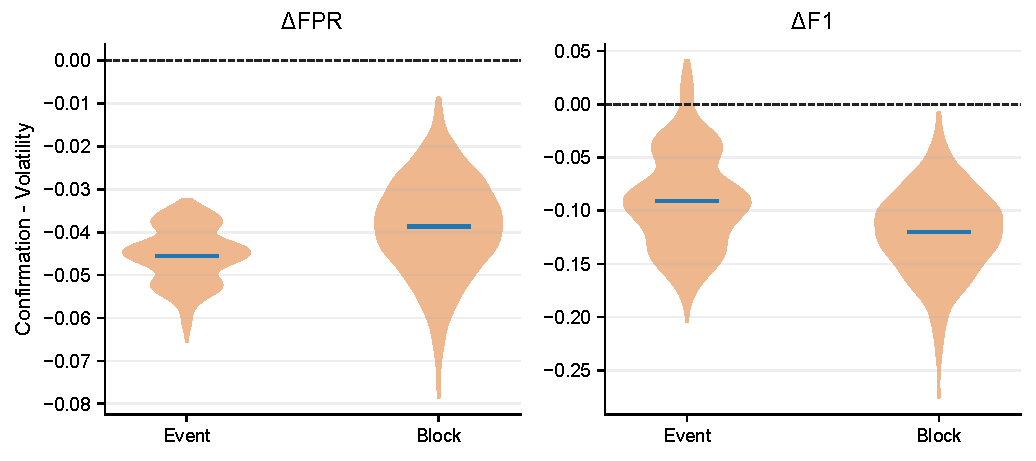
\includegraphics[width=0.50\textwidth]{Fig8.pdf}
\caption{Bootstrap distributions of the difference between the confirmation rule and the volatility trigger.}
\label{fig:bootstrap_violin}
\end{figure*}

\subsection{Synthetic and NAB checks}
The generated series in Figure~\ref{fig:synthetic_example} contains stable, drift, and collapse regimes with heavy-tailed noise. Detector outputs follow the regime changes, which shows that the pipeline responds to them in the generator.

On NAB, mean F1 is 0.141 for the confirmation rule and 0.140 for the volatility trigger, while the false positive rate is 0.105 against 0.141. This matches the SPY pattern, where confirmation reduces false positives without raising F1. Figure~\ref{fig:nab_results} gives the breakdown by subset. The NAB path replaces MMD with a rolling mean-difference statistic, so it evaluates a different confirmation rule under the same metrics and checks the scoring code rather than reproducing the SPY detector.

\begin{figure*}[t]
\centering
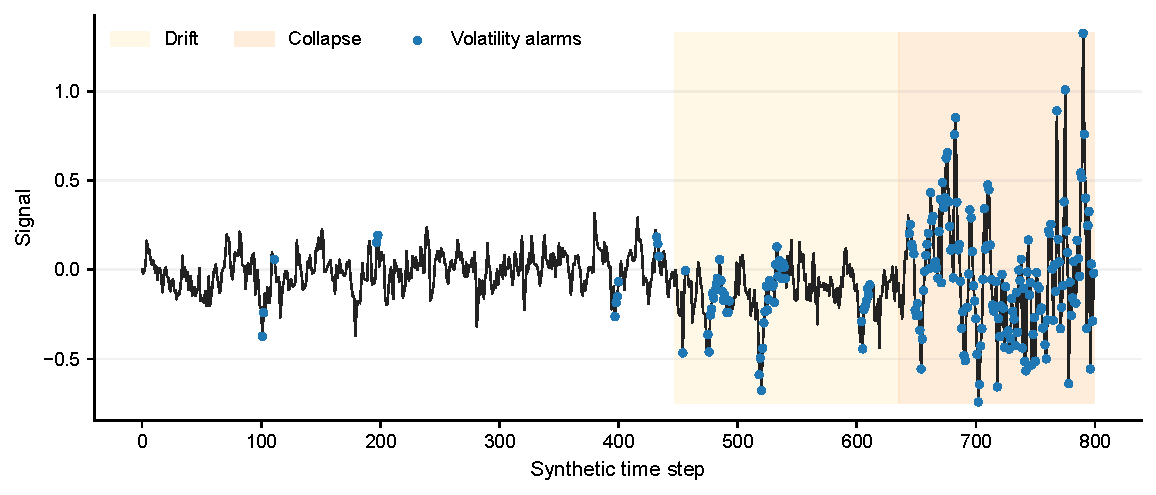
\includegraphics[width=0.75\textwidth]{Fig9.pdf}
\caption{Generated series with regime changes and the resulting detector outputs.}
\label{fig:synthetic_example}
\end{figure*}

\begin{figure*}[t]
\centering
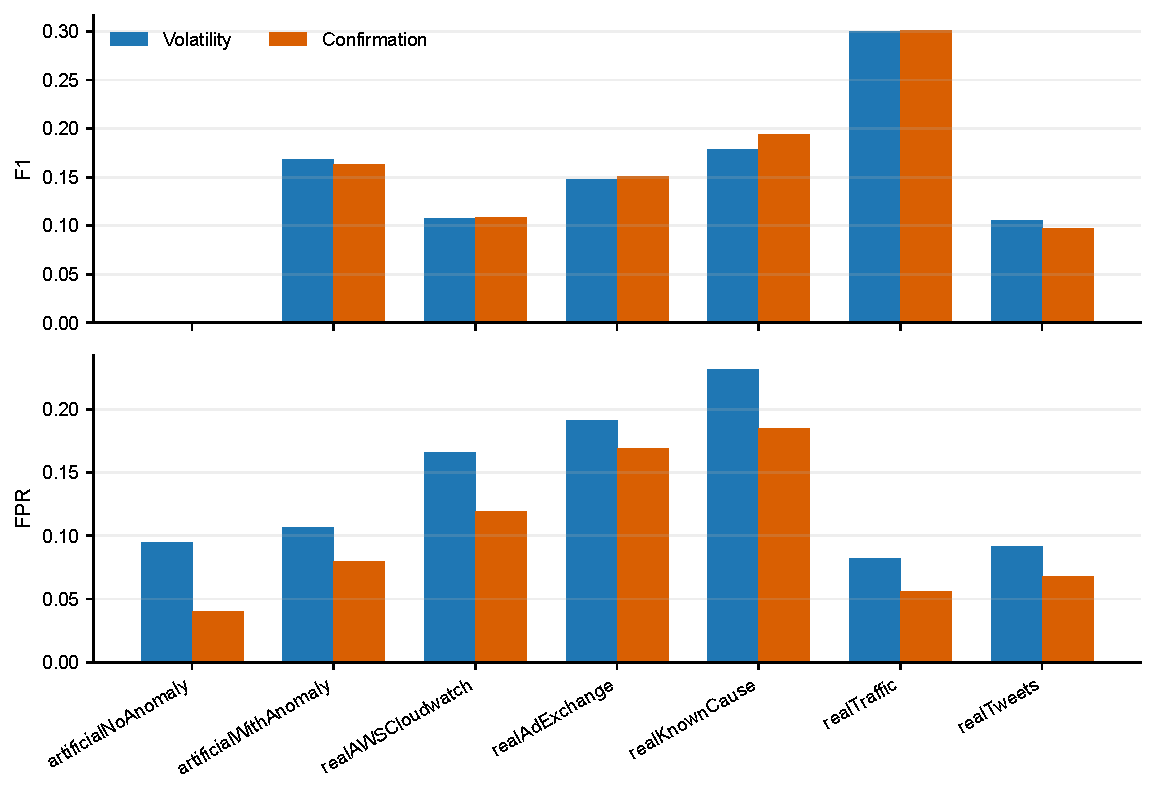
\includegraphics[width=0.75\textwidth]{Fig10.pdf}
\caption{NAB results by subset, using the same day-level metrics as the stress protocol.}
\label{fig:nab_results}
\end{figure*}

\begin{table*}[t]
\centering
\caption{NAB F1 and false positive rate by subset.}
\scriptsize
\setlength{\tabcolsep}{2pt}
\begin{tabular}{lrrrr}
\toprule
Subset & Vol. F1 & Vol. FPR & Confirm. F1 & Confirm. FPR\\
\midrule
artificialNoAnomaly & 0.000 & 0.095 & 0.000 & 0.040\\
artificialWithAnomaly & 0.168 & 0.107 & 0.163 & 0.080\\
realAWSCloudwatch & 0.108 & 0.166 & 0.108 & 0.119\\
realAdExchange & 0.148 & 0.191 & 0.151 & 0.169\\
realKnownCause & 0.179 & 0.232 & 0.194 & 0.185\\
realTraffic & 0.300 & 0.082 & 0.302 & 0.056\\
realTweets & 0.106 & 0.092 & 0.097 & 0.068\\
\bottomrule
\end{tabular}
\end{table*}

\section{Discussion}
\label{sec:discussion}
The same two alarm series produce opposite rankings under the day-level metrics and under the event-level metrics. The confirmation rule raises precision from 0.640 to 0.886 and lowers the false positive rate from 0.044 to 0.005, while it detects 8 of the 13 events instead of 10, lowers recall from 0.225 to 0.122, and moves the mean first alarm from 1.2 trading days before the event to 6.8 days after it. A single F1 value reports none of this. CUSUM shows the same problem: it has the highest F1 in Table~\ref{tab:spy}, 0.364, together with a false positive rate of 0.344, because it alarms on much of the sample and those alarms fall inside the wide event windows.

The ranking reverses because of the input the confirmation condition reads. That input divides each return by the standard deviation of the previous 50 days. The condition therefore responds when a return is large compared with that standard deviation. When volatility rises slowly enough, the standard deviation rises with it, and the condition does not respond. On the U.S. downgrade the volatility condition holds on 49 window days and the instability condition on 1; on the 2022 inflation selloff the counts are 40 and 2. This is a property of the input rather than of the threshold. Widening the confirmation window from 10 to 60 days raises F1 to 0.291 and the false positive rate to 0.031, and still leaves the U.S. downgrade undetected; the inflation selloff is picked up from $W=30$ onward, at a sixfold rise in the false positive rate. A confirmation layer intended to detect such events needs an input that is not divided by a trailing standard deviation.

The two detectors therefore fit different uses. A monitoring system can accept a higher false positive rate in return for detecting more events and detecting them earlier. A layer whose alarms are followed by manual review cannot, since each alarm costs analyst time. The crossover ratio states where the boundary between the two lies: on SPY the volatility trigger costs less only when one alarm day outside the windows costs less than 0.021 of a missed event, and across the five assets and three delay penalties the boundary lies between 0.007 and 0.059. The ranking is the same under every parameter value tested: at all four event-window widths, under all ten weightings of the composite signal, and under both one-sided versions of the persistence term. It rests on a margin of 2 events on a panel of 13, so the SPY counts alone are weak evidence; the same ordering appears on all five assets, and the bootstrap supports the difference in false positive rate more firmly than the difference in F1.

\section{Limitations}
\label{sec:limits}
\begin{itemize}
\item \textbf{Panel.} The 13 episodes are U.S. equity events. International crises, sector-specific disruptions, and most credit and liquidity events are absent, and a wider panel could change the detection rates.
\item \textbf{Severity.} Severity is the realized SPY drawdown around each date, split at terciles of 13 values. It describes realized impact within this panel, is not a validated scale, and is applied to the other four assets unchanged.
\item \textbf{Assets.} Five exchange-traded funds are used. Individual equities, non-U.S. indices, commodities, currencies, and macroeconomic indicators are not covered, and neither detector is presented as the best available.
\item \textbf{Auxiliary checks.} The synthetic series are not calibrated to market data. The NAB check uses non-financial data, a faster substitute for the MMD statistic, and our metrics rather than NAB's own scoring.
\item \textbf{Uncertainty and cost.} The bootstrap holds the detector outputs fixed, covers SPY only, and cannot compensate for a panel of 13 events. The cost model is deliberately simple, and its parameters are settings rather than measured quantities.
\item \textbf{Mechanism.} The explanation rests on two missed events on one asset, supported by a synthetic test. It has not been checked on a large set of real events.
\item \textbf{Use of future data.} The trailing and causal variants are evaluated on SPY only, and a causal replacement for the MMD statistic is untested.
\end{itemize}

\section{Reproducibility and Code Availability}
\label{sec:repro}
The code and data needed to reproduce every result are available at \url{https://github.com/prashant290605/Financial-stress-event-fixed-protocol}. The package contains the event panel with its per-asset mapped dates and sources, the archived price series used here, all detector and evaluation settings, and the random seed. Every reported result uses seed 42 and thresholds calibrated on the first 70 per cent of each series. The script \texttt{scripts/run\_ablations.py} regenerates Tables~\ref{tab:mechanism}, \ref{tab:crossover}, \ref{tab:weights}, \ref{tab:kappasign}, and \ref{tab:causal}, and \texttt{scripts/run\_synthetic\_mechanism.py} regenerates the synthetic test. The remaining results come from \texttt{scripts/run\_vix\_benchmark.py} for Table~\ref{tab:vix}, \texttt{scripts/evaluate\_multi\_asset.py} for Table~\ref{tab:multiasset_pointwise}, \texttt{scripts/evaluate\_event\_level.py} for Tables~\ref{tab:spy_event_level}, \ref{tab:multiasset_event_level}, and \ref{tab:event_level_severity}, and \texttt{scripts/run\_cost\_analysis.py} for Table~\ref{tab:event_cost}. The repository lists requirements, expected runtimes, output locations, and known limits on reproduction.

\section{Conclusion}
\label{sec:conclusion}
The day-level metrics and the event-level metrics rank the two detectors in opposite orders. On SPY the confirmation rule lowers the false positive rate from 0.044 to 0.005, raises precision from 0.640 to 0.886, and costs less at every day-level weighting tested. Measured against the fixed events, it detects 8 of the 13 rather than 10, its recall falls from 0.225 to 0.122, and it confirms the Lehman episode 40 trading days later than the volatility trigger. Both sets of figures are correct. Reporting only one of them is what this protocol is designed to prevent. The cause lies in the input to the confirmation condition, which divides each return by a trailing standard deviation. The condition responds when a return is large compared with that standard deviation, and not when volatility rises slowly enough for the standard deviation to rise with it. On the two episodes the confirmation rule alone misses, the volatility condition holds on 49 and 40 window days and the instability condition on 1 and 2, and a test on generated data reproduces the same behaviour on constructed episodes. Any confirmation layer built on such an input misses the same episodes, and its low false positive rate depends on reading days after the alarm.

The crossover ratio turns this into a figure a user can apply. On SPY the volatility trigger costs less only when one false-alarm day costs less than 0.021 of a missed episode, that is, when a missed episode is worth more than 48 false-alarm days. Across the five assets the crossover lies between 0.007 and 0.059. A user can compare that figure with their own costs and choose a detector, which is more useful than a single ranking.

\backmatter

\section*{Statements and Declarations}

\bmhead{Acknowledgements}
The authors thank the Department of Mathematics, Indian Institute of Technology Ropar, for institutional support.

\bmhead{Author Contributions}
Prashant Singh: conceptualization, methodology, software, formal analysis, and writing of the original draft. Pranav Singh: methodology, validation, interpretation of results, and review and editing. Both authors approved the final manuscript.

\bmhead{Funding}
The authors received no funding for this work.

\bmhead{Data Availability}
Daily prices for SPY, QQQ, IWM, HYG, and TLT and daily VIX closing levels were retrieved from Yahoo Finance (SPY on 30 March 2026, the other assets on 22 May 2026, VIX on 22 July 2026) and are archived with the code, together with the event panel and its sources.

\bmhead{Code Availability}
Code and reproducibility materials are available at \url{https://github.com/prashant290605/Financial-stress-event-fixed-protocol}.

\bmhead{Use of Artificial Intelligence}
The authors used generative artificial intelligence for assistance with manuscript formatting and language. The authors reviewed and edited the resulting text and are responsible for the study design, analyses, results, and interpretations.

\bmhead{Competing Interests}
The authors declare no competing interests.

\bmhead{Ethics Approval and Consent to Participate}
Not applicable. The study did not involve human participants, human data, human tissue, or animals.

\bmhead{Consent for Publication}
Not applicable.

\begin{appendices}
\renewcommand{\theHtable}{A.\arabic{table}}
\renewcommand{\theHfigure}{A.\arabic{figure}}
\renewcommand{\theHequation}{A.\arabic{equation}}

\section{Implementation details}
\label{app:implementation_details}
The event panel is in \texttt{data/events\_spy.csv} and its per-asset mapped version in \texttt{data/events\_multi\_asset.csv}. All detector, evaluation, and bootstrap settings, and the random seed, are in \texttt{config/paper\_experiment.json}. Most reported results are regenerated by \texttt{scripts/reproduce\_paper.py}; the tables it does not produce are listed with their scripts in Section~\ref{sec:repro}. Table~\ref{tab:asset_availability} gives the usable sample for each series and Table~\ref{tab:hyperparams} the settings used.

\begin{table*}[t]
\centering
\caption{Usable daily sample for each series after preprocessing.}
\label{tab:asset_availability}
\scriptsize
\begin{tabular}{llrr}
\toprule
Series & Description & Dates & Days\\
\midrule
SPY & S\&P 500 ETF & 2000-03-15--2023-12-29 & 5987\\
QQQ & Nasdaq 100 ETF & 2000-03-15--2023-12-29 & 5987\\
IWM & Russell 2000 ETF & 2000-08-08--2023-12-29 & 5886\\
HYG & High-yield bond ETF & 2007-06-21--2023-12-29 & 4161\\
TLT & Treasury bond ETF & 2002-10-09--2023-12-29 & 5343\\
VIX & Cboe Volatility Index & 2000-03-15--2023-12-29 & 5987\\
\bottomrule
\end{tabular}
\end{table*}

\noindent The VIX snapshot covers 6037 trading days. It is aligned to the SPY calendar and used as a level rather than a return, so the evaluation uses SPY's 5987 processed days.

\begin{table*}[t]
\centering
\caption{Detector and evaluation settings.}
\label{tab:hyperparams}
\scriptsize
\begin{tabular}{p{0.18\linewidth}p{0.76\linewidth}}
\toprule
Component & Setting \\
\midrule
Preprocessing & Log returns; 20-day volatility; 50-day standardized return; composite $x_t=0.5r_t+0.3\sigma_t+0.2z_t$.\\
Calibration & First 70\% of each series; 90th percentile thresholds.\\
Volatility trigger & Standardized $\sigma_t$; five-day trailing mean; 90th percentile threshold.\\
CUSUM & Standardized returns; two-sided recursion with no drift term; five-day trailing mean; 90th percentile threshold.\\
MMD & Two samples of 30 observations; RBF kernel; median pairwise distance as bandwidth, floored at $10^{-4}$.\\
Persistence $\kappa$ & Trailing 36 days; $\kappa_t=1-\widehat\phi_t$; two-sided $|z_\kappa|$ by default.\\
Confirmation rule & $W=10$ trading days; volatility condition on day $t$ and instability condition within $[t-W,t+W]$.\\
Bootstrap & 2000 resamples; event rows or overlapping 20-day blocks; 95\% percentile intervals.\\
Ablations & Ten weightings $(w_r,w_\sigma,w_z)$; confirmation term $|z_\kappa|$, $\max(-z_\kappa,0)$, or $\max(+z_\kappa,0)$.\\
\bottomrule
\end{tabular}
\end{table*}

Synthetic data are used only as a diagnostic, and no setting is carried from them to the market analysis. Labels come from three regimes: stable, drift, and collapse. The generated signal is
\begin{equation}
x_t=0.7\,x_{t-1}+d_t-\beta x_{t-1}^{3}+\epsilon_t,
\end{equation}
\begin{equation}
\epsilon_t=\sigma_t u_t+\ell_t,
\end{equation}
where $u_t$ is Student-$t$ noise, $\ell_t$ is Laplace noise, $d_t<0$ is a drift term active in the drift regime, and $\sigma_t$ is raised during stress and near collapse. Table~\ref{tab:synthetic_params} lists the settings.

\begin{table}[t]
\centering
\caption{Synthetic generator settings.}
\label{tab:synthetic_params}
\scriptsize
\begin{tabular}{lr}
\toprule
Parameter & Value or range\\
\midrule
Series & 30\\
Length & 800\\
Student-$t$ df & [3, 8]\\
Laplace scale & [0.01, 0.05]\\
Calm volatility & [0.005, 0.02]\\
Stress multiplier & [1.5, 4.0]\\
Drift magnitude & [-0.08, -0.02]\\
Nonlinear $\beta$ & [0.01, 0.08]\\
\bottomrule
\end{tabular}
\end{table}

For NAB, all 58 series in \texttt{combined\_windows.json} are used. The labelled windows are converted to daily masks and no parameter is tuned. To keep the run tractable across all 58 series, this path replaces the exact MMD computation with a rolling mean-difference statistic.

\section{Dispersion around events}
\label{app:mechanism}
For each event, the dispersion ratio is the standard deviation of a series inside the $\pm60$ trading-day window divided by its standard deviation over the 120 trading days before the window. Raw 20-day volatility is not divided by any trailing scale, while $x_t$ is, through the 50-day standardization in $z_t$.

Across the seven detected events with a full 120-day preceding window, the mean ratio is 3.03 for raw volatility and 1.29 for $x_t$. The dot-com selloff is excluded, since it lies too near the start of the processed series to have a full preceding window.

The two events missed only by the confirmation rule show the two ways the condition fails. For the U.S. downgrade the ratios are 3.26 and 1.24 and peak smoothed $z_{\mathrm{MMD}}$ is 0.96: volatility expanded, and the trailing 50-day scale absorbed it. For the 2022 inflation selloff the ratios are 1.11 and 0.85 and peak $z_{\mathrm{MMD}}$ is 1.84: volatility was already high through 2022, so the two 30-day samples compared by the kernel statistic were alike.

\end{appendices}

\bibliography{sn-bibliography}
\end{document}
